\documentclass[]{spie}  %>>> use for US letter paper
%%\documentclass[a4paper]{spie}  %>>> use this instead for A4 paper
%%\documentclass[nocompress]{spie}  %>>> to avoid compression of citations
%% \addtolength{\voffset}{9mm}   %>>> moves text field down
%% \renewcommand{\baselinestretch}{1.65}   %>>> 1.65 for double spacing, 1.25 for 1.5 spacing 
%  The following command loads a graphics package to include images 
%  in the document. It may be necessary to specify a DVI driver option,
%  e.g., [dvips], but that may be inappropriate for some LaTeX 
%  installations. 
\usepackage[]{graphicx}
\usepackage{subfigure}
\usepackage{amsmath}
\usepackage{hyperref}

\graphicspath{{images/}}

\title{CIVILITY: Cloud based Interactive Visualization of Tractography Brain Connectome} 

\author{Dana\"{e}le Puechmaille\supit{a}, Martin Styner\supit{a} and Juan C. Prieto\supit{a}
\skiplinehalf
\supit{a}Neuro Imaging Reasearch and Analysis Laboratory, Department of Psychiatry, \\
 University of North Carolina, Chapel Hill, North Carolina, United States;
}

%>>>> Further information about the authors, other than their 
%  institution and addresses, should be included as a footnote, 
%  which is facilitated by the \authorinfo{} command.

\authorinfo{Further author information: (Send correspondence to J.C.P)\\J.C.P.: E-mail: jprieto@med.unc.edu\\D.P: E-mail:danaele@email.unc.edu\\M.S.: styner@cs.unc.edu}
%%>>>> when using amstex, you need to use @@ instead of @
 

%%%%%%%%%%%%%%%%%%%%%%%%%%%%%%%%%%%%%%%%%%%%%%%%%%%%%%%%%%%%% 
%>>>> uncomment following for page numbers
 \pagestyle{plain}    
%>>>> uncomment following to start page numbering at 301 
%\setcounter{page}{301} 
 
  \begin{document} 
  \maketitle 

%%%%%%%%%%%%%%%%%%%%%%%%%%%%%%%%%%%%%%%%%%%%%%%%%%%%%%%%%%%%% 
\begin{abstract}

Cloud based Interactive Visualization of Tractography Brain Connectome (CIVILITY) is an interactive visualization tool of brain connectome in the cloud. This application submits tasks to remote computing grids were the CIVILITY-tractography pipeline is deployed. 
The application will list the running tasks for the user and once a task is completed the brain connectome is visualized using Hierarchical Edge Bundling. 
The analysis pipeline uses FSL tools (bedpostx and probtrackx2) to generate a triangular matrix indicating 
the connectivity strength between different regions in the brain.
This work is motivated by medical applications in which expensive computational tasks such as brain connectivity is needed and to provide 
a state of the art visualization tool of Brain Connectome. 

This work does not contribute any novelty with respect to the visualization methodology, is rather a new resource for the neuroimaging community.
This work is submitted to the SPIE Biomedical Applications in Molecular, Structural, and Functional Imaging conference. 
The source code of this application is available in NITRC\footnote{\url{http://www.nitrc.org/projects/civility}}

\end{abstract}

%>>>> Include a list of keywords after the abstract 

\keywords{Tractography, connectivity, diffusion tensor imaging, brain connectome, cloud, open source, application}

%%%%%%%%%%%%%%%%%%%%%%%%%%%%%%%%%%%%%%%%%%%%%%%%%%%%%%%%%%%%%
\section{INTRODUCTION}
\label{sec:intro}

Tractography is used to enhance our knowledge of human brain anatomy. Recent studies analyzed pediatric subjects with longitudinal data
in order to understand the development trend of fibers in the infant brain\cite{10.1371/journal.pone.0024678}. 
Progress has been made to develop visualization tools that will help researches better understand brain connectivity\cite{10.1371/journal.pone.0068910}. 
Nevertheless, there is an opportunity to develop new tools for brain connectome visualization.
In this paper, we present CIVILITY, an open source web application to visualize the brain connectome.  
This tool offers researchers the possibility to submit the tractography pipeline to remote computing grids 
and to visualize the results of the brain connectome in an interactive plot.
The tractography pipeline uses the probabilistic method of tractography using surfaces as seeds \cite{Behrens2007144}\cite{MRM:MRM10609}. 
This expensive computational task is executed on a remote computing grid and once completed, the brain connectome can be visualized 
in a circular plot known as Hierarchical Edge Bundling plot implemented using Data Driven Documents (D3.js)
CIVILITY uses clusterpost\footnote{https://www.npmjs.com/package/clusterpost-server} to submit the task to remote computing grids. 
CIVILITY provides the interface to set the inputs for the brain connectivity pipeline and clusterpost 
is in charge of submitting the task, monitoring its completion and retrieving the results. 
Once a taks is completed, CIVILITY provides the option to retrieve the results or visualize them directly in the circular plot
or displayed on top of a brain template. 

This work does not contribute any novelty with respect to the visualization methodology, is rather a new resource for the community.
This work is submitted to the Biomedical Applications in Molecular, Structural, and Functional Imaging conference. 

In order to validate this tool, we applied the tractography pipeline to a set of infant brains. 
The following section explains in detail the methods used in CIVILITY.

\section{METHODS} 
\label{sec:METHODS}

The figure \ref{fig:architectureCIVILITY} shows the architecture of the application CIVILITY. 

\begin{figure}
\centering 
\includegraphics[width=15cm]{architectureCIVILITYOut.eps}
\caption[Architecture of the application CIVILITY]{Architecture of the application CIVILITY. }
\label{fig:architectureCIVILITY}
\end{figure}

The following section explains the necessary input parameters to start the tractography pipeline. 

\subsection{Tractography}

\subsubsection{Input parameters}

To start the tractography pipeline, the following parameters are needed: Diffusion Weighted Image (DWI), T1 image, brain mask, a parcellation table
and white matter surface. If the white matter surface does not contain information about the brain regions, 
the gray matter containing labeled regions can be added as well. 
For a detailed explanation about the input parameters, please visit the main repository of the application\footnote{https://github.com/NIRALUser/CIVILITY}.

The following section explains the CIVILITY-tractography pipeline.

\subsubsection{CIVILITY-Tractography pipeline}

CIVILITY-tractography pipeline uses FSL tools, a comprehensive library of analysis tools for FMRI, MRI and DTI brain imaging data developed by the Analysis group \footnote{https://fsl.fmrib.ox.ac.uk/fsl/fslwiki}.
The tool uses a Bayesian Estimation of Diffusion Parameters Obtained using Sampling Techniques for modeling Crossing Fibers (bedpostx). 
This tool builds up distributions on diffusion parameters at each voxel in the image and prepares it to run probabilistic tractography. 
The utility ExtractLabelSurfaces\footnote{https://github.com/NIRALUser/ExtractLabelSurfaces} will extract each surface region and will update a seed list to start the tractography. 

Finally, probtrackx2 runs the probabilistic tractography, using the outputs from bedpostx and ExtractLabelSurfaces. 
The outputs of this pipeline yields a triangular matrix indicating the strength of connectivity between each brain region.
The connectivity values range from 0 or no connectivity to 1 full connectivity.

Next section explains how the resulting triangular matrix is visualized.

\subsection{Visualization}

CIVILITY-visualization will generate the brain connectome using the results from the pipeline described above.
The visualization requires the connectivity matrix and a parcellation table describing the brain atlas in brain surfaces. 

The brain connectome is plotted using a circle plot know as Hierarchical Edge Bundling. 
The visualization offers the possibility to display the minimum, maximum or average between the lower or upper sides of the matrix. 
A tension value can be set in order to change the shape of the links and facilitate visualization. 

The interactive visualization allows the user to threshold the output matrix between two values. 
The strength of the link between regions is colored using a rainbow gradient. 

The following section explains the materials used to compute the tractography. 

\section{MATERIALS}

We apply our tractography pipeline to 19 infants (scanned at 1 year and 2 years approximately).
All data passed Quality Control (QC) and was registered in the same physical space of the DWI image. 
The surface used for this analysis contained label information according to the brain atlas Automated Anatomical Labeling (AAL90).
The following section shows the results of this pipeline. 

\section{RESULTS} 

We compute the brain connectome of these 19 infants at years 1 and 2. The input surfaces for the tractography overlap with each other. 
The cerebellum regions are ignored in the brain connectome computation. The number of samples is set to 3000 (number of streamlines per voxel) with a step length of 0.75mm and a seed sphere sampling of 0.5. 

\subsection{Brain connectome average}

The connectivity is computed with the average value between the lower and upper triangles of the connectivity matrix.
The resulting matrices from 19 infants are averaged as shown in equation \ref{equ:average}.

\begin{equation}
	A_{i,j} = \frac{\sum_{i=0}^n M_i}{n}
	\label{equ:average}
\end{equation}



\begin{figure}
\centering 
\subfigure[]{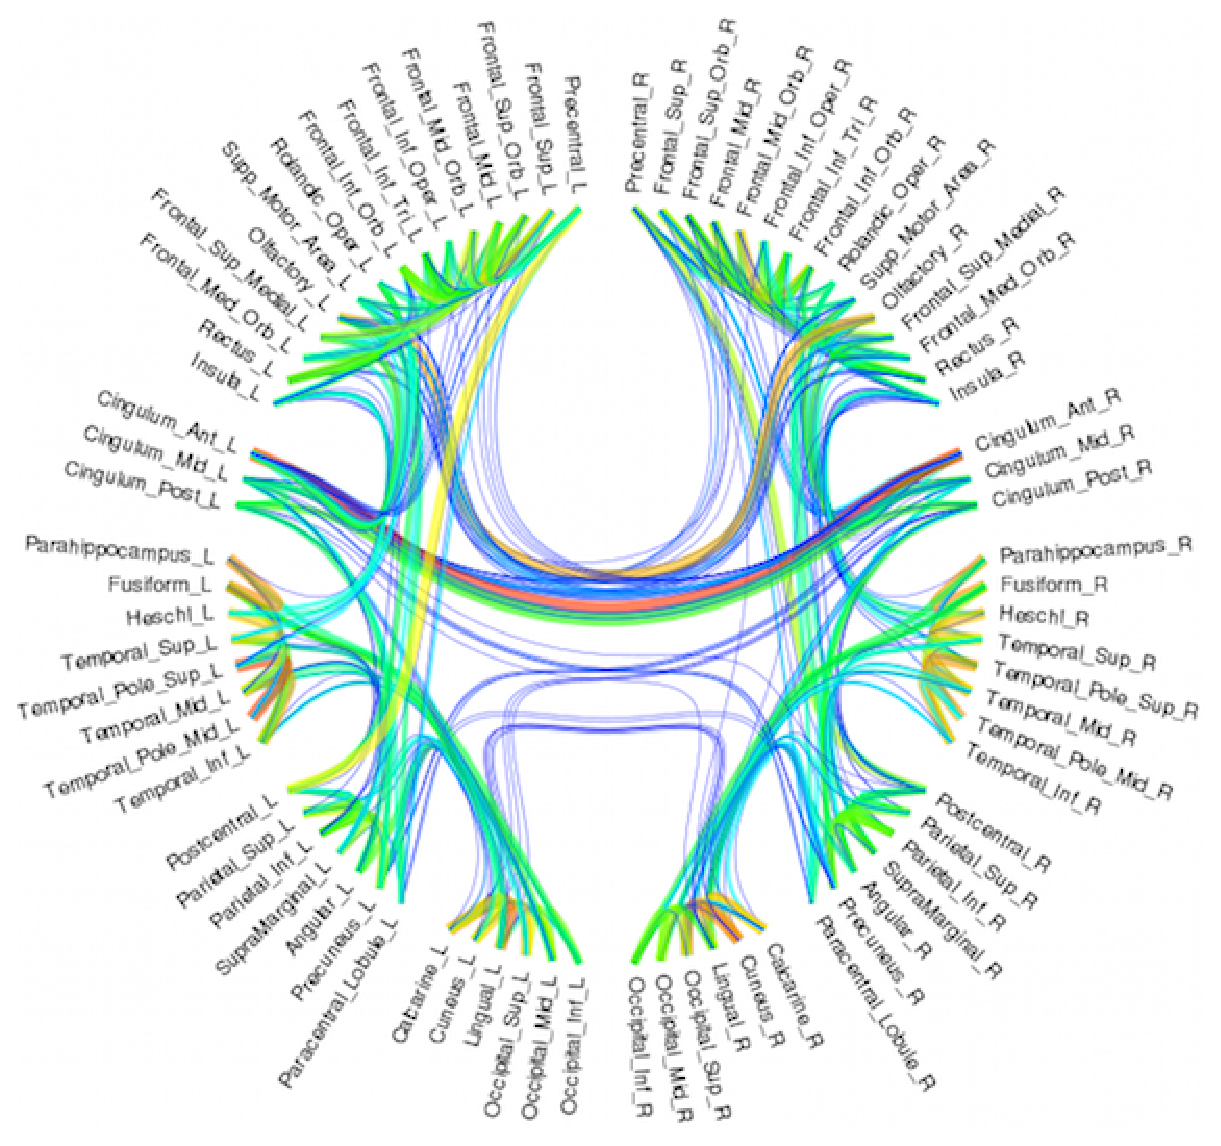
\includegraphics[width=8cm]{average_1yOut.eps}}
\subfigure[]{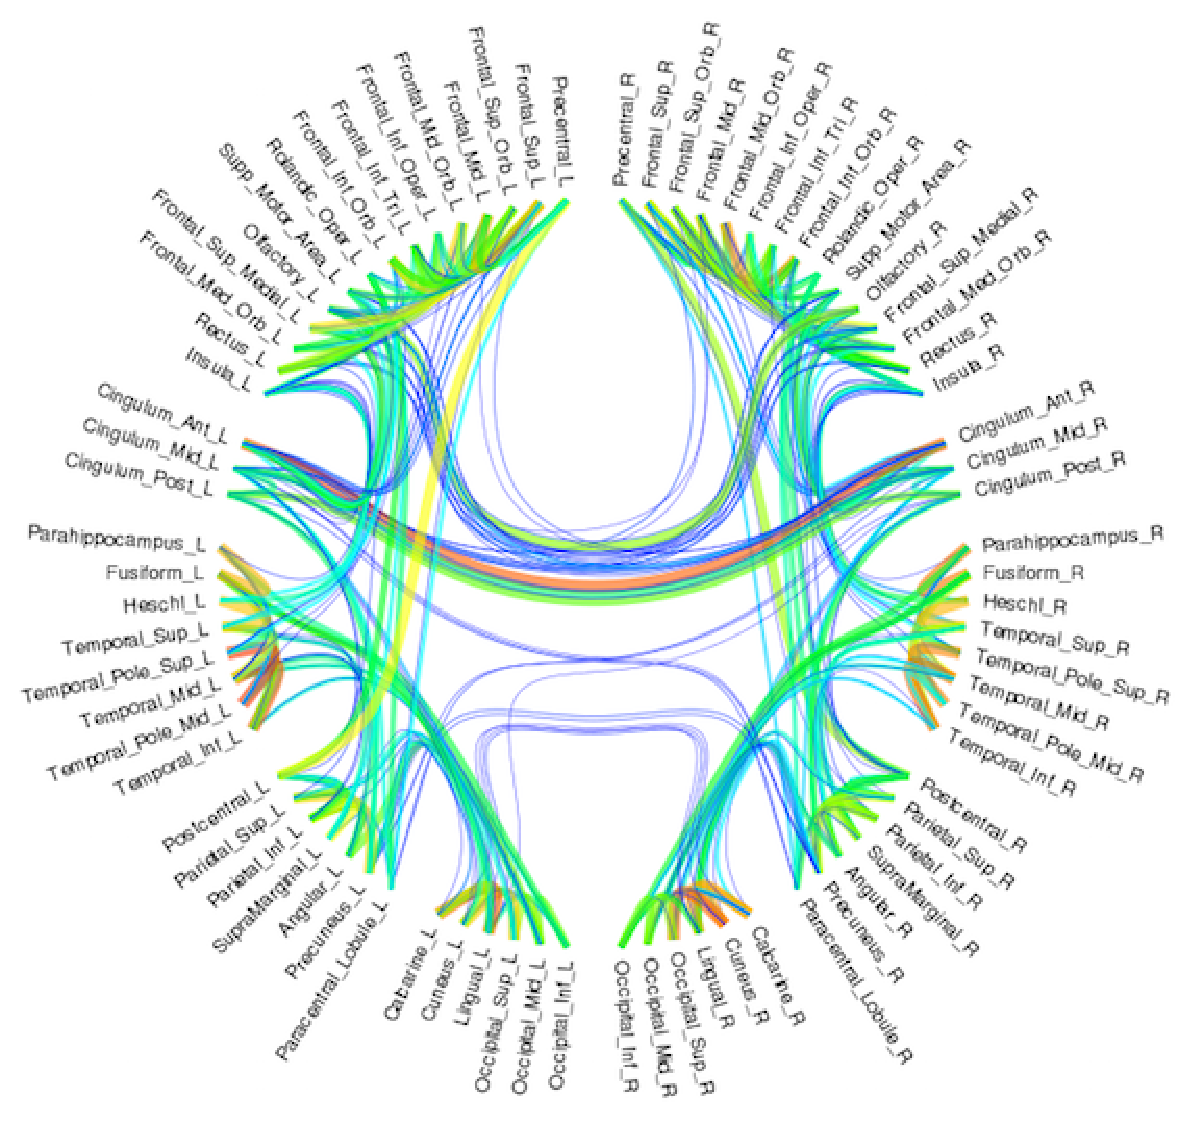
\includegraphics[width=8cm]{average_2yOut.eps}}
\subfigure{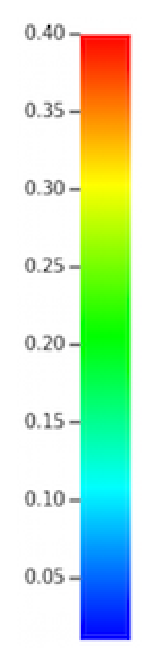
\includegraphics[width=0.9cm]{colorbarAverage1y2yOut.eps}}
\subfigure[]{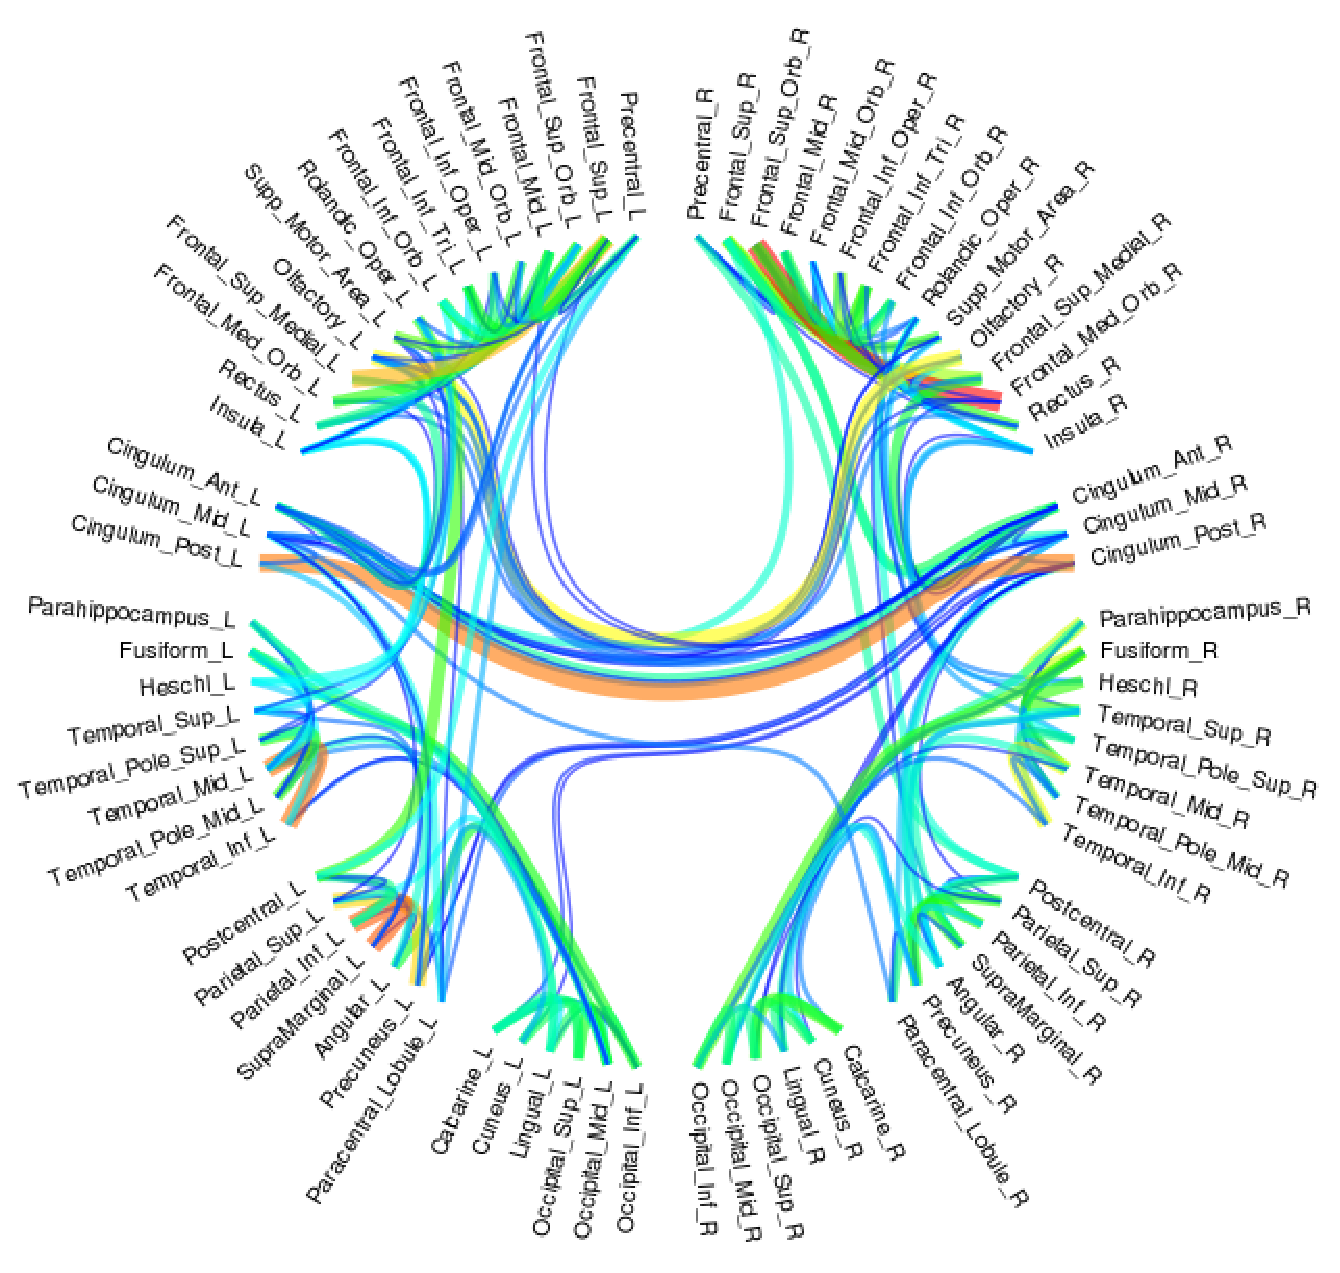
\includegraphics[width=8cm]{variance_1yOut.eps}}
\subfigure[]{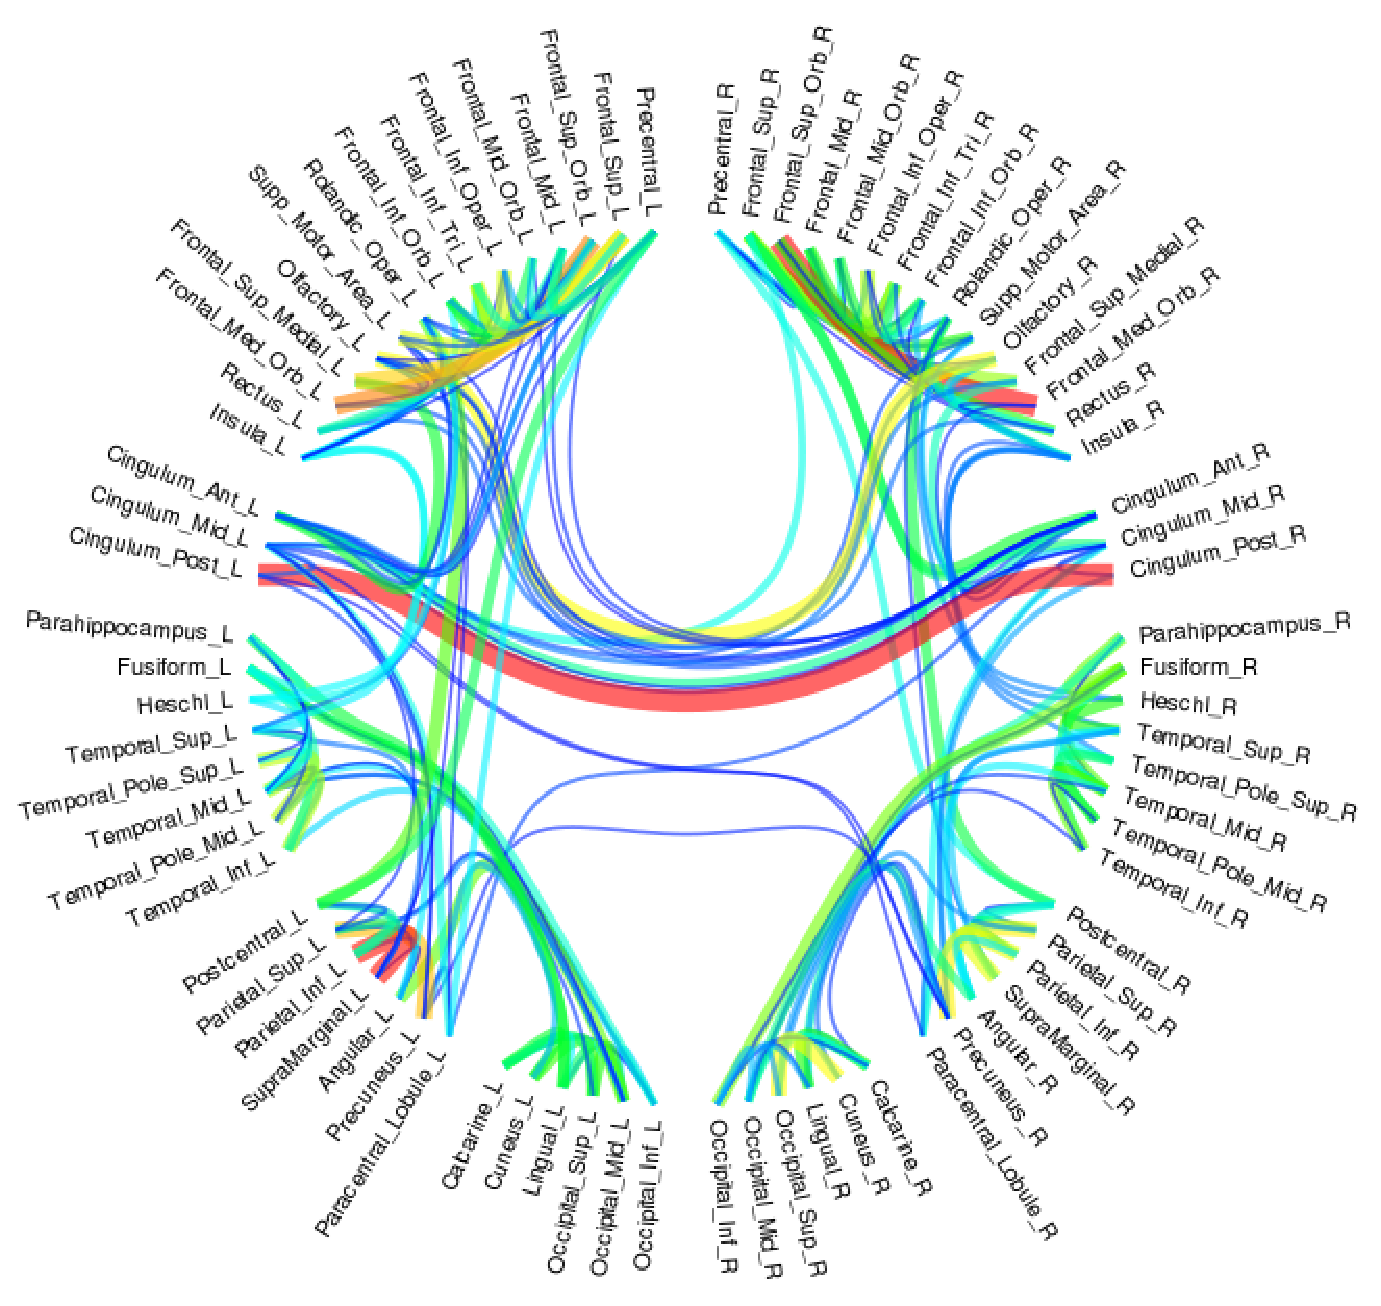
\includegraphics[width=8cm]{variance_2yOut.eps}}
\subfigure{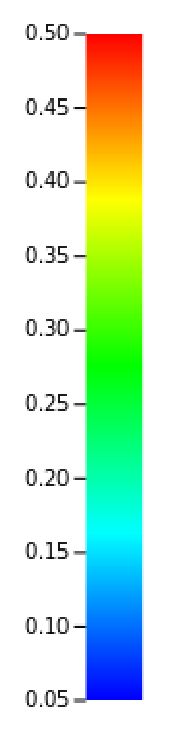
\includegraphics[width=0.9cm]{variance_1y_2y_colorbarOut.eps}}
\caption[Average brain connectome at 1 (a) and 2 (b) year old using the circle plotting ]{Figures (a) and (b) show the average brain connectome with threshold 
[0.01 - 0.4] for 1 and 2 years old respectively. Figures (d) and (e) use a threshold [0.05 - 0.5]. }
\label{fig:AverageBrainConnectome}
\end{figure} 

Figure \ref{fig:AverageBrainConnectome} shows the average brain connectome for 1 year and 2 year old infants using different thresholds. We threshold the plotting using two ranges, i.e., [ 0.05, 0.5 ] and [0.04, 0.4 ] for better visualization.

These results show a variability pretty constant between 1 and 2 year old, but higher at 2 years old.
Figures \ref{fig:AverageBrainConnectomeBrainTemplate} shows the average brain connectome visualized on a brain template with threshold [0.01 - 0.4].

\begin{figure}
\centering 
\subfigure[]{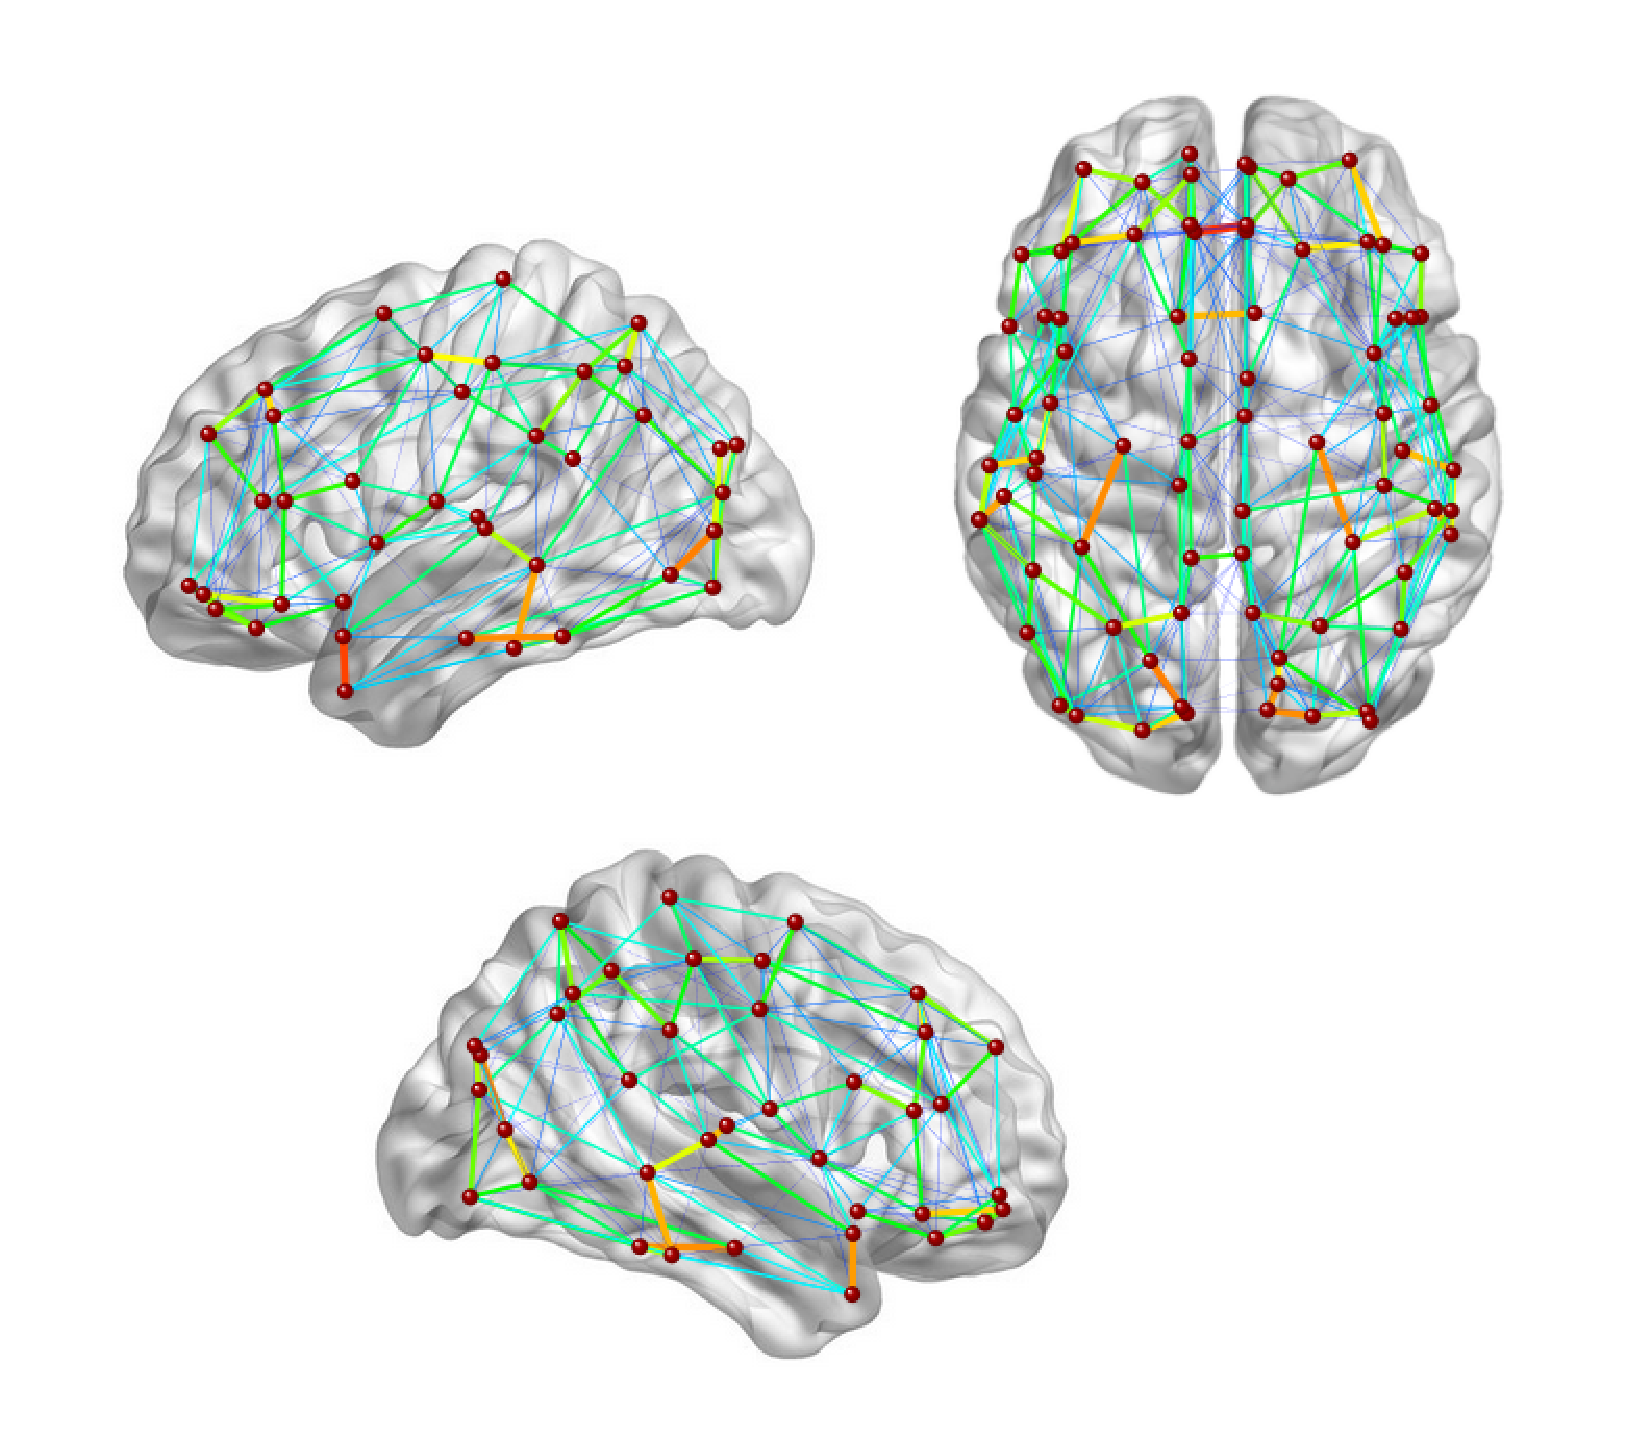
\includegraphics[width=8cm]{average_brainTemplate_1yOut.eps}}
\subfigure[]{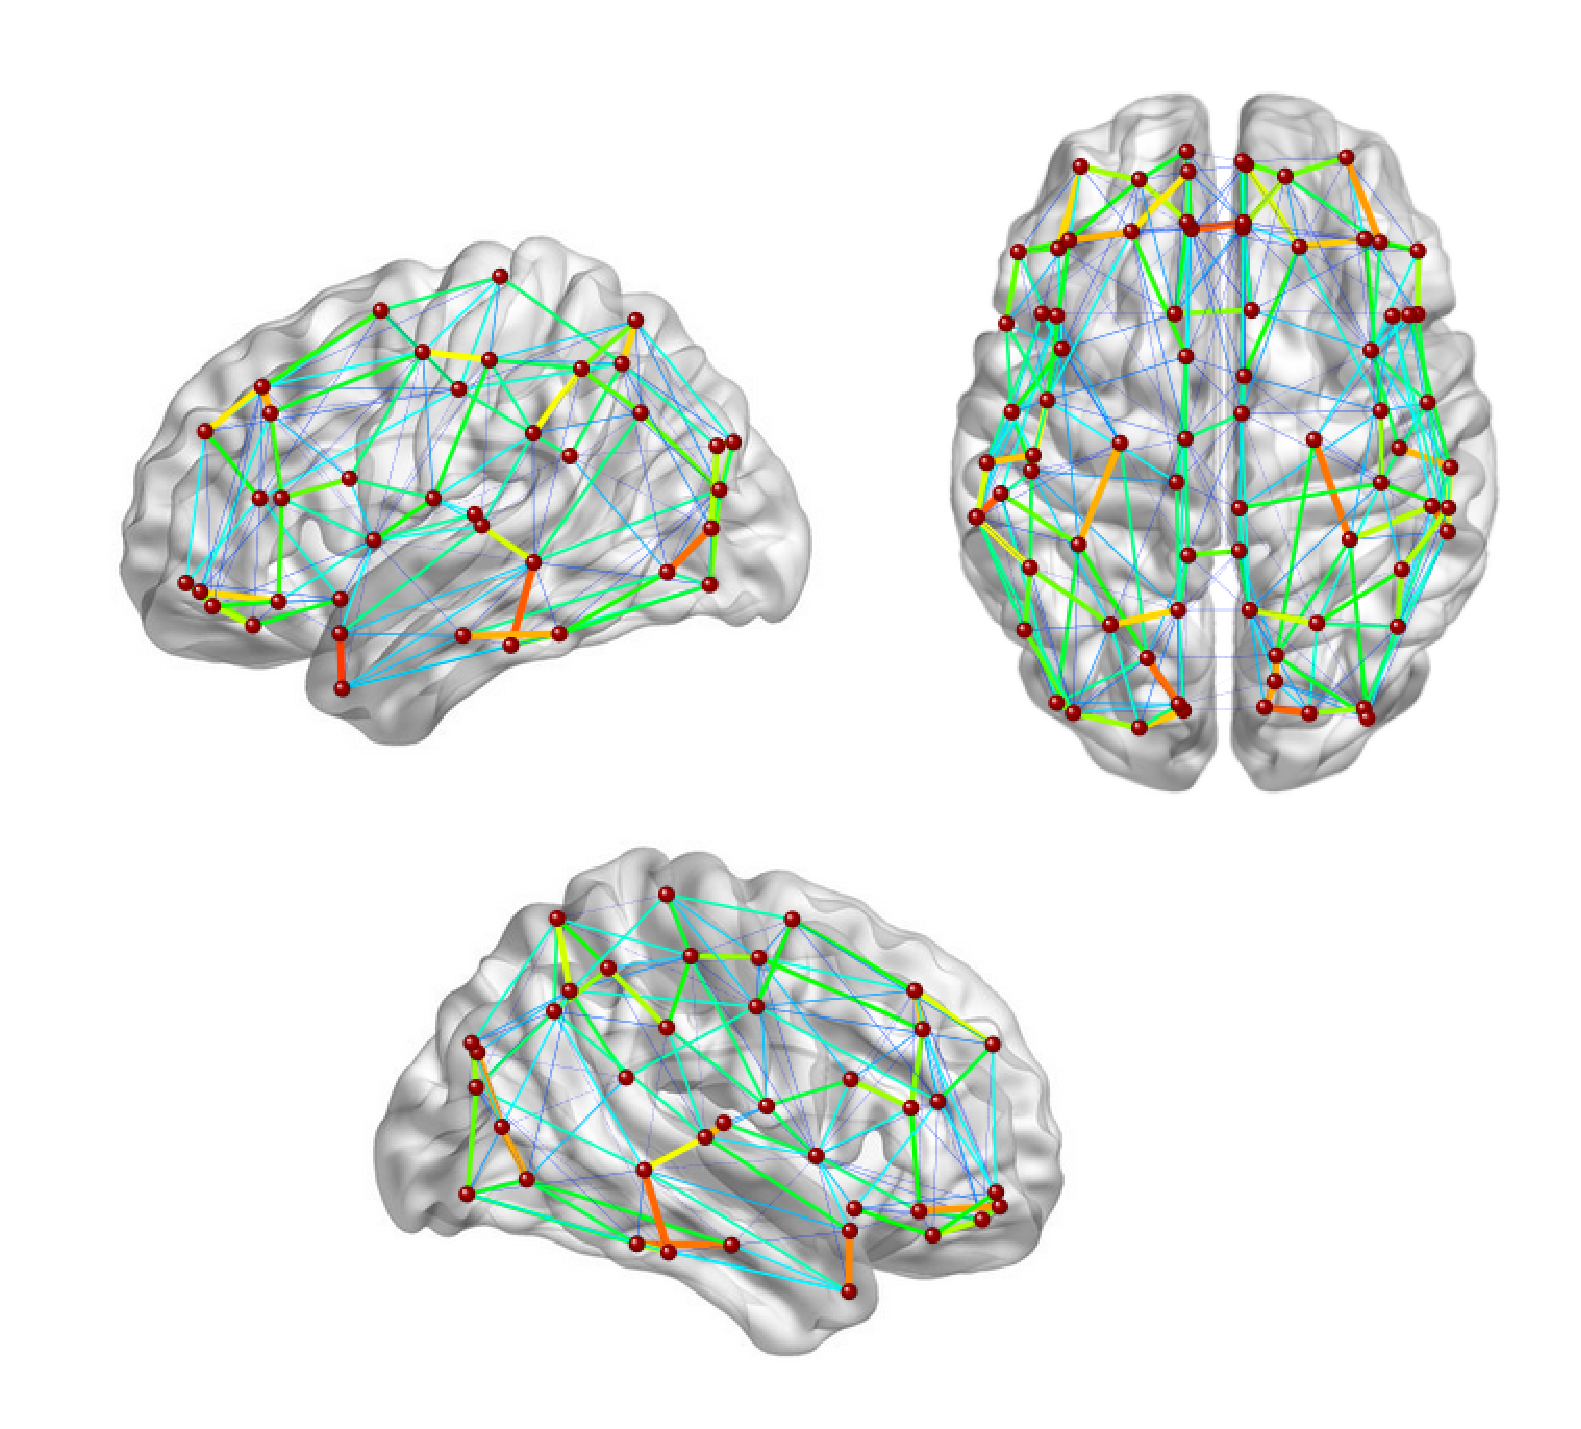
\includegraphics[width=8cm]{average_brainTemplate_2yOut.eps}}
\caption[Average brain connectome at 1 (a) and 2 (b) year old on brain templates ]{Average brain connectome at 1 (a) and 2 (b) year old on brain templates. Threshold : 0.01 - 0.4}
\label{fig:AverageBrainConnectomeBrainTemplate}
\end{figure} 

The shape of the connectivity is similar at both ages. However, some links are missing in the brain connectome for 1 year old subjects and the connectivity values are lower for 1 year old children when compared to 2 year old children.

\subsection{Variability and deviation of the brain connectome}

We compute the unbiased sample variance as shown in Equation \ref{equ:unbiasedSampleVariance} to show the variability of the brain connectome in a dataset. The resulting matrix is visualized. 

\begin{equation}
	V_{i,j} = \frac{1}{n-1} \times \sum_{i=0, j=0}^n {(M_{i,j} - A_{i,j})^2}
	\label{equ:unbiasedSampleVariance}
\end{equation}

We also compute the standard deviation of this dataset at 1 and 2 year old (Equation \ref{equ:standardDeviation}).

\begin{equation}
	D_{i,j} = \sqrt{V_{i,j}}
	\label{equ:standardDeviation}
\end{equation}

\begin{figure}
\centering 
\subfigure[]{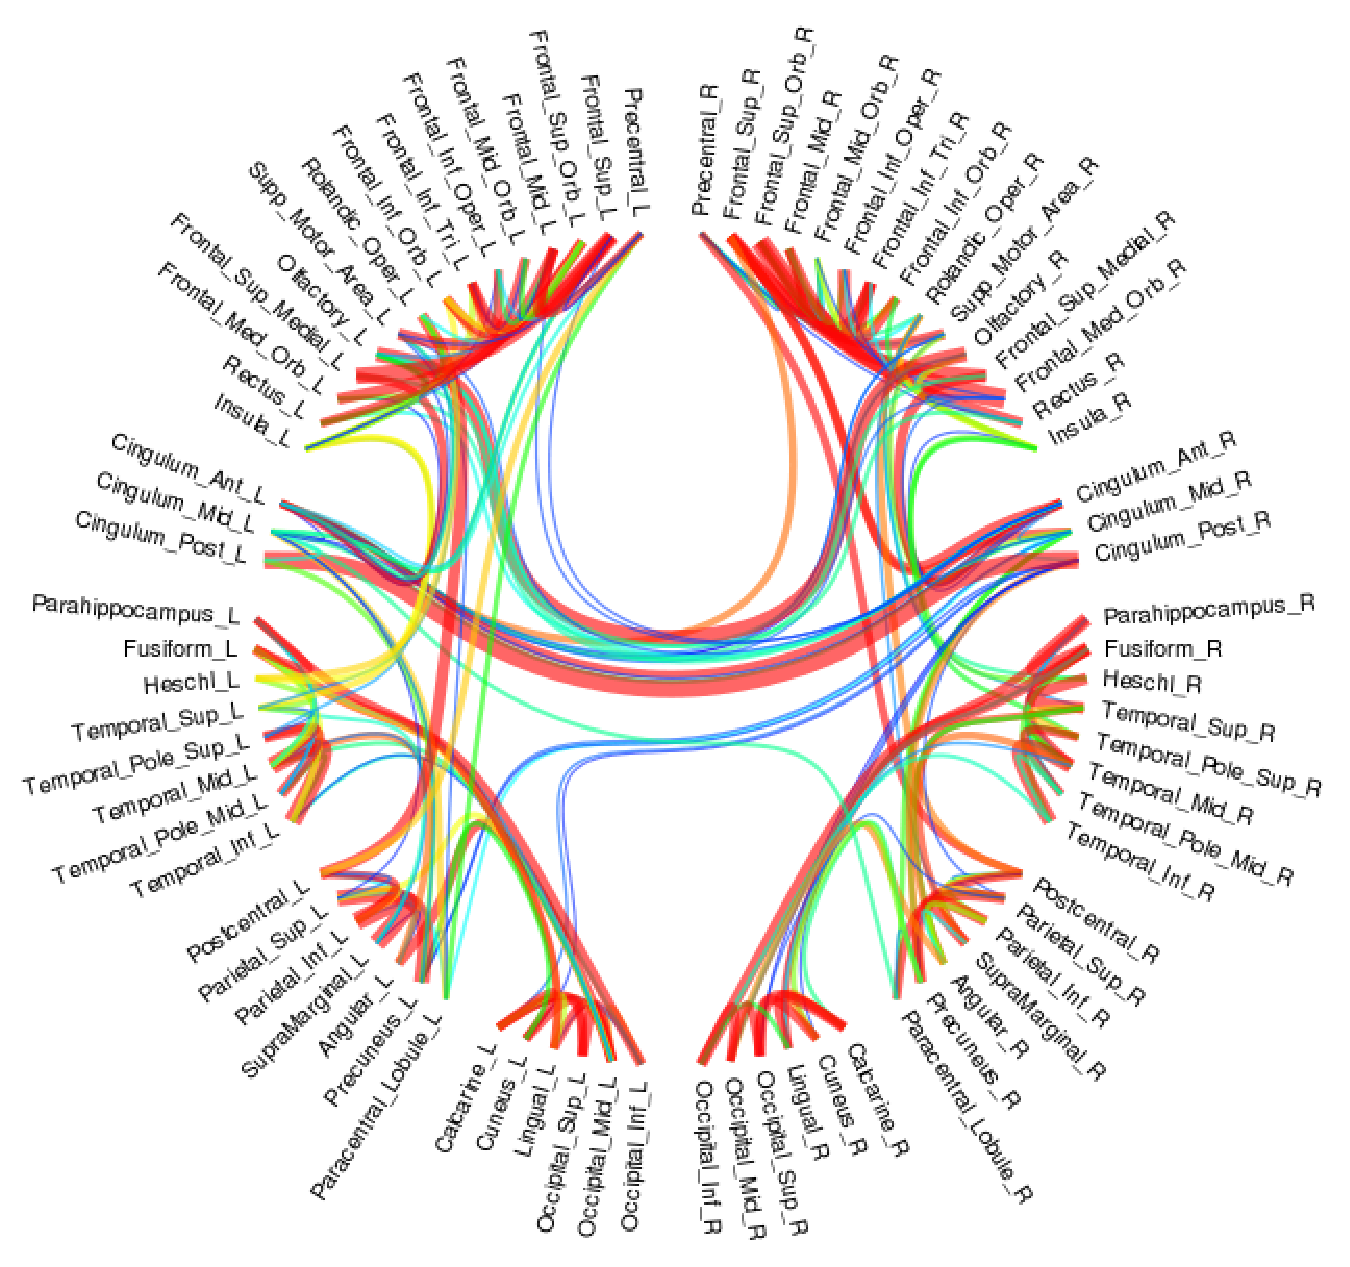
\includegraphics[width=8cm]{deviation_1yOut.eps}}
\subfigure[]{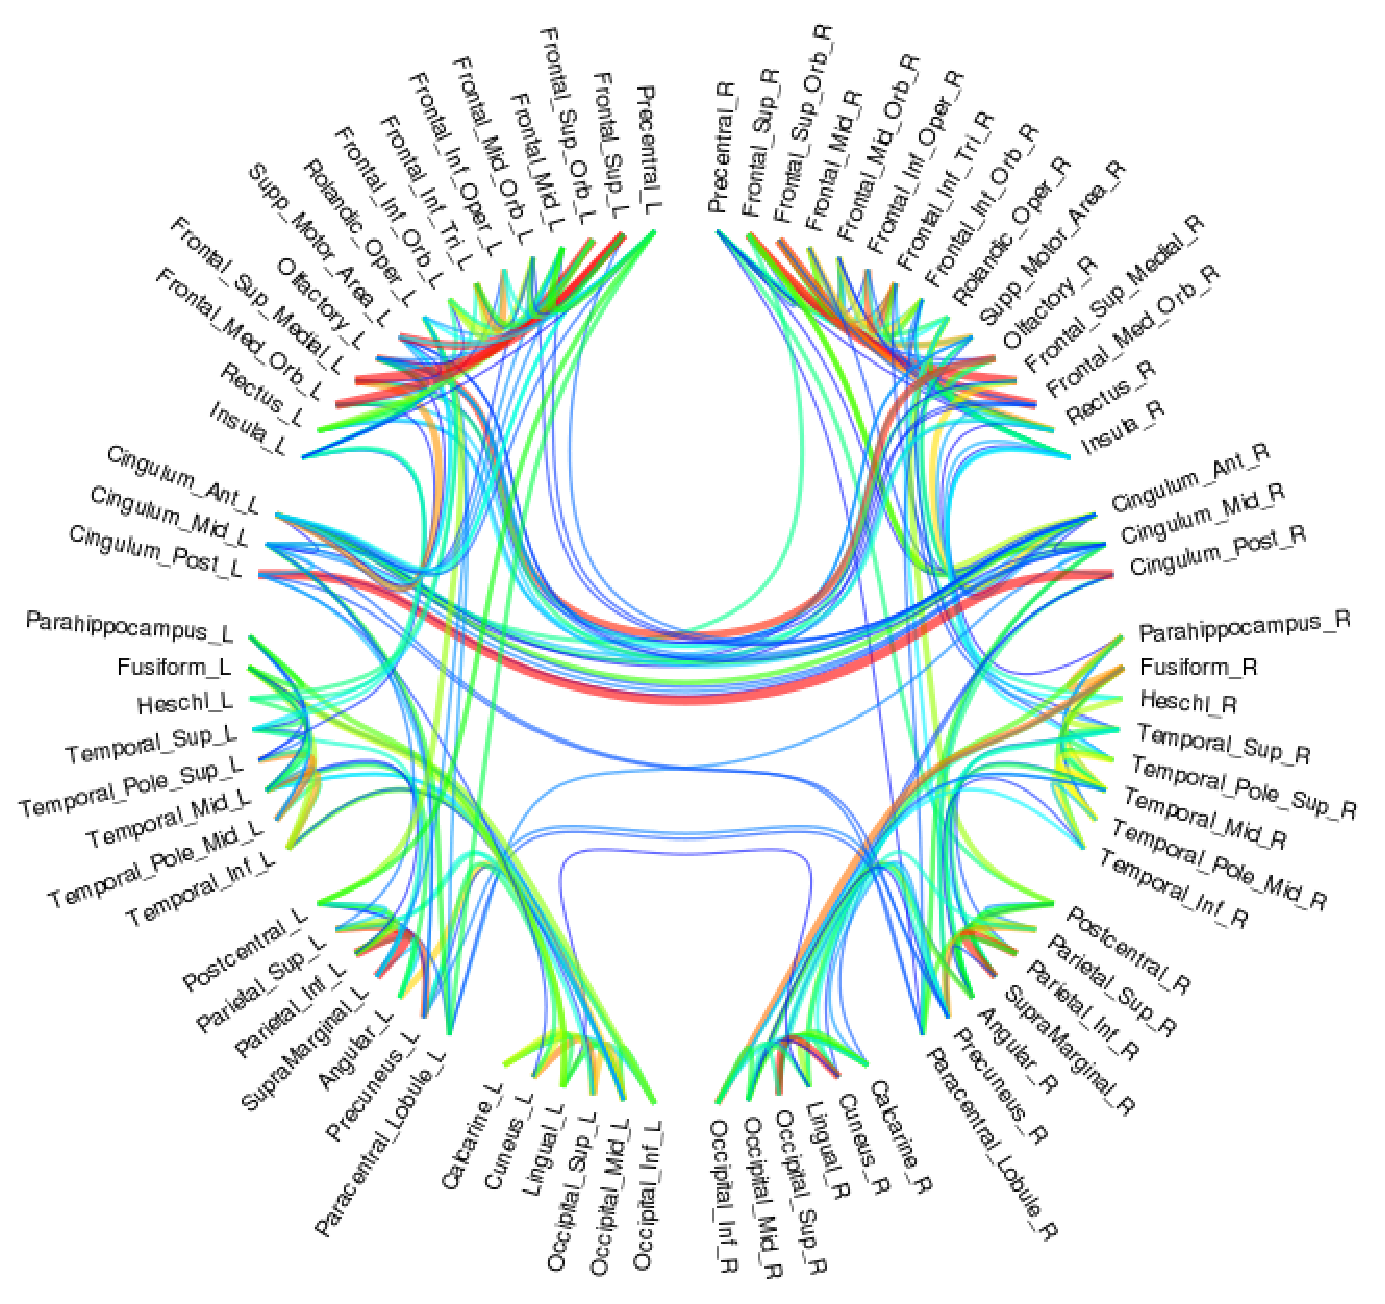
\includegraphics[width=8cm]{deviation_2yOut.eps}}
\subfigure{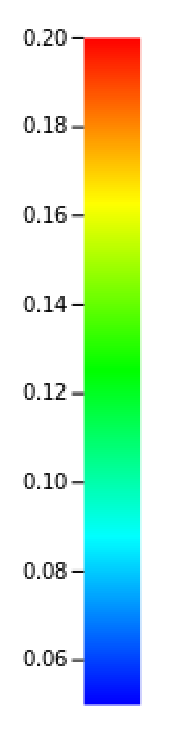
\includegraphics[width=0.9cm]{deviation_1y_2y_colorbarOut.eps}}
\caption[Standard deviation of the brain connectome at 1 (a) and 2 (b) year old on brain templates ]{Standard deviation of the brain connectome at 1 (a) and 2 (b) year old on brain templates. Threshold : 0.05 - 0.2}
\label{fig:DeviationBrainConnectome}
\end{figure} 

Figure \ref{fig:DeviationBrainConnectome} shows the deviation in the brain connectome. 
We threshold between 0.05 and 0.2 for better visualization. The image shows higher variability for 1 year old infants. The deviation for 2 year old infants is much lower. 

\section{CONCLUSIONS} 

We presented CIVILITY, Cloud based Interactive Visualization of Tractography Brain Connectome which is a web application running in the cloud. 
CIVILITY offers the possibility to the users to launch a tractography pipeline in remote computing grids. 
Data transfer and task monitoring are handled by the application. 
Running a brain tractography task in a computing grid is desirable 
as it may take up to one week to finish processing a single subject. 
Once completed, the results are made available to the user for visualization. 

We have developed an interactive visualization using Hierarchical Edge Bundling,
This type of graph facilitates the representation of complex data such as brain connectivity between regions. 
With this user-friendly tool for brain connectome, we expect to 
enhance our understanding of brain development during childhood and reduce the time consuming 
operation when a study requires processing multiple subjects. 

This tool does not contribute any novelty with respect to methodology, 
but is rather a new resource for the community. This work is submitted to the Biomedical Applications in Molecular, Structural, and Functional Imaging conference. The source code of this application is available here\footnote{\url{http://www.nitrc.org/projects/civility}}.


\acknowledgments

Thanks to Dr. Guilmore, UNC, for use of his dataset. Grants: UO1MH070890, U54HDO79124, RO1MH091351. 

%%%%%%%%%%%%%%%%%%%%%%%%%%%%%%%%%%%%%%%%%%%%%%%%%%%%%%%%%%%%%
%%%%% References %%%%%

\bibliography{report}   %>>>> bibliography data in report.bib
\bibliographystyle{spiebib}   %>>>> makes bibtex use spiebib.bst

\end{document} 
